\subsection{Preprocesamiento y limpieza de datos para el Reconocimiento de Patrones}

El preprocesamiento de datos es una etapa fundamental en el reconocimiento de 
patrones, ya que garantiza la calidad y relevancia de los datos antes de su 
análisis. Este proceso incluye varias técnicas como limpieza, transformación, 
reducción y normalización de datos. La limpieza de datos implica la eliminación de 
valores atípicos, datos incompletos o inconsistentes, mientras que la tranformación 
convierte los datos en un formato adecuado, como la codificación de variables 
categóricas o la aplicación de transformaciones matemáticas. La normalización y 
estandarización aseguran que los datos tengan una escala uniforme, lo cual es 
crucial para algoritmos que dependen de medidas de distancia. Además, en el caso de 
datos textuales o de imágenes, se aplican técnicas específicas como la tokenización 
o el filtrado de ruido. Un buen preprocesamiento no solo mejora la precisión de los 
modelos de reconocimiento de patrones, sino que también reduce el tiempo de 
procesamiento y evita problemas de sobreajuste.

En este proceso se aplican diferentes técnicas de análisis de datos que van desde
la visión por computadora hasta el procesamiento de señales biomédicas. Las 
principales técnicas utilizadas en el preprocesamiento de datos son:

\begin{itemize}
    \item Limpieza de datos. Consiste en eliminar errores, valores atípicos y datos 
    faltantes para asegurar la calidad de los datos antes de su uso en modelos de 
    reconocimiento de patrones. Las principales funciones son: el manejo de valores 
    faltantes, eliminación de outliers y corrección de inconsistencias.
    
    \item Normalización y estandarización. Este conjunto de funciones aseguran 
    que las características tengan escalas comparables, mejorando la estabilidad y 
    rendimiento de los algoritmos de reconocimiento de patrones, entre los principales 
    métodos se encuentran la normalización (Min-Max Scaling), estandarización y escalamiento.
    
    \item Transformaciones de datos. Mejora la representación de los datos para aumentar 
    la capacidad predictiva y mejorar la separación entre clases. Estas transformaciones 
    pueden ir desde transformación logarítmica y raíz cuadrada, hasta transformadas de 
    Fourier y Wavelet, así mismo se suele utilizar una codificación 
    One-Hot que convierte variables categóricas en vectores binarios y la codificación de 
    frecuencia que asigna valores numéricos en función de la frecuencia de aparición de una 
    categoría.
    
    \item Filtrado y eliminación de ruido. Se aplica principalmente en señales e imágenes 
    para mejorar la calidad de los datos y facilitar su análisis. Algunos de los filtros 
    que se utilizan son: filtros de suavizado, filtro Notch, filtro pasa bajas y pasa altas. 
    
    \item Integración y formateo de datos. Cuando se utilizan múltiples fuentes de datos, 
    es escencial integrarlas y formatearlas de manera coherente. Algunas de las técnicas 
    que podemos utilizar  para esto son: la conversión de fotmatos que transforma los tipos 
    de datos para compatibilidad con diferentes herramientas de análisis y la reducción de 
    redundancia que utilizamos para la eliminación de información duplicada para evitar 
    sesgos en el análisis. 

\end{itemize}

\subsection{ECG (electrocardiograma)}

La señal electrocardiográfica (ECG) es un registro de la actividad eléctrica del corazón 
y se utiliza ampliamente en el diagnóstico de enfermedades cardiovasculares. El ECG está 
compuesto por diversas ondas, incluyendo la onda P, el complejo QRS y la onda T, que reflejan 
la despolarización y repolarización del corazón. Existen diversos métodos para el análisis de 
la señal ECG, como la descomposición en Fourier, que permite separar sus componentes y mejorar 
la interpretación de los datos. Sin embargo, las señales ECG pueden estar contaminadas con ruido, 
como interferencias de línea de alimentación y artefactos de movimiento, lo que requiere técnicas 
de filtrado para mejorar la calidad del análisis. Además, el desarrollo de algoritmos de 
clasificación, ha permitido mejorar la detección de patologías cardíacas a partir de la señal ECG.

\begin{figure}[H]
    \centering
    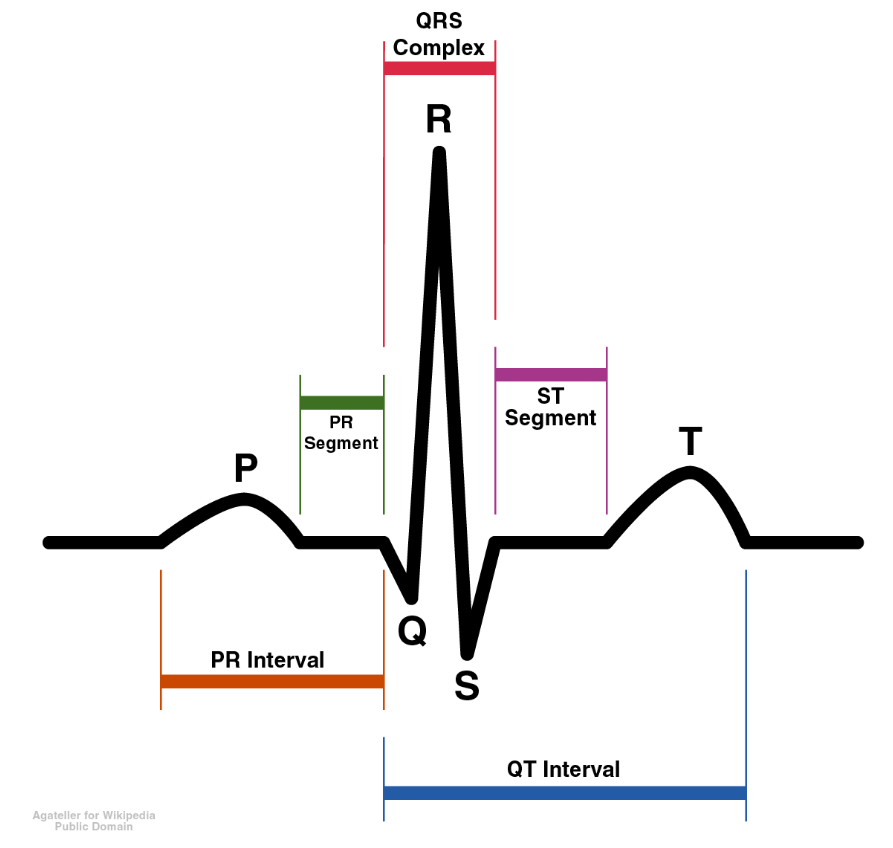
\includegraphics[width = 0.6\textwidth]{Img/ECG.png}
    \caption{Representación esquemática de un ECG normal.}
    \label{fig:placeholder}
\end{figure}